\chapter[Revisión de literatura]{Marco Teórico}

\subsection[Reseña Histórica]{Reseña Histórica}
Para empezar a adentrarnos a los conceptos del Procesamiento de Lenguaje Natural primero
empezaremos a repasar hitos importantes en áreas de conocimiento afines.
% https://www.cs.bham.ac.uk/~pjh/sem1a5/pt1/pt1_history.html
Los primera aplicación reconocida como una NPL fueron en 1948 que fue un buscador de palabras en el
diccionario de desarrollado en Birkbeck College de Londres por Warren Weaver. Luego rápidamente
surgió como idea de investigación crear una maquina de traducción automática en varios grupos de en
Estados Unidos, Reino Unido, Francia y Rusia. Los primeros grupos se concentraron en traducir texto
en Alemán, cuando los textos de la Segunda Guerra Mundial se volvieron obsoletos, pasaron a el Ruso
el mayor problema fue que no existían todavía fundamentos formales de al computación, ni mucho
menos de NLP. La mayoría de los investigadores eran matemáticos e inmigrantes bilingües que
intentaban encontrar relaciones entre ambos lenguajes. La investigación concluyo en que todavía no
existían los recursos necesarios para abordar dicho problema, pero se desarrollaron mejoras en
herramientas para la traducción asistida.\cite{hancox}
%  Sumit raj
En 1950 Alan Turing desarrolla el test de Turing que es un test para distinguir el nivel de
inteligencia de una maquina, propuso que un humano evaluara las conversaciones en un lenguaje
natural entre un humano y una máquina diseñada para dar respuestas similares a los humanos. Lo que
pudo definir la inteligencia de un sistema de cómputo de una forma comparable a la inteligencia
humana.
En el año 1954 un experimentó de colaboración de la Georgetown University e IBM se  hace publica la
primera demostración logra la traducción automática de mas de 60 se oraciones en Ruso al Ingles.
Las oraciones eran previamente elegidas que trataban de temas políticos, legales, matemáticos y
científicos. Luego eran ingresados a la maquina escritos en Ruso con letras romanizadas. El método
era principalmente lexicográfico basado en un diccionario de relaciones de palabras de ambos
idiomas.\cite{ibm_2003}
En las décadas posteriores se siguieron dando avances con métodos basados en reglas algorítmicas
como arboles de decisión para el procesamiento del lenguaje y la traducción automática. A partir de
los 2000s la investigación se centro en algoritmos de Machine Learning no supervisados y semi
supervisados, por amplia disponibilidad de información no clasificados en literatura e internet,
por lo general estos métodos son menos eficientes que los algoritmos supervisados pero la cantidad
de datos existentes pueden equiparar estas deficiencias. En la segunda década del nuevo milenio se
utilizaron nuevos métodos basados en Aprendizaje de características y Deep Learning lo que nos trae
al estado actual del arte que discutiremos en la siguiente sección.

\section[Procesamiento de lenguaje natural]{Procesamiento de lenguaje natural (NPL)}
El procesamiento de lenguaje natural o por sus siglas en inglés NPL(de natural language processing)
es un campo de las Ciencias de Computación y la Lingüística que trata con métodos para analizar,
modelar y entender el lenguaje humano.

%---usar sownya vajja Practical Natural Language Processing_ A Comprehensive Guide to Building Real como referencia

\subsection{Lenguaje}% que es un lenguaje, fonemas, syntaxis, etc 
Primero de los conceptos claves para poder adentrarnos a  NLP es definir el Lenguaje, un Lenguaje
es un sistema de comunicación que involucra una combinación compleja de componentes como, letras,
palabras, etc. La Lingüística es el estudio sistemático del lenguaje. Para poder estudiar NLP, es
importante entender componentes del lenguaje.\cite{sowmya_practical_npl}
\begin{figure}[h]
	\centering
	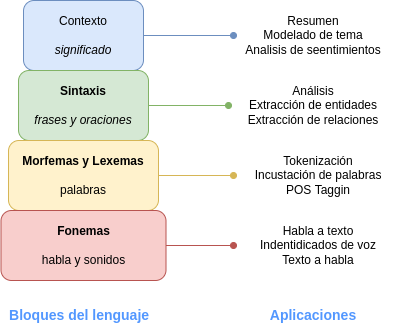
\includegraphics[width=\textwidth]{imagenes/Cap 2/lenguaje.drawio.png}
	\caption{Aplicaciones de partes de un Lenguaje}
	\label{fig:Aplicaciones de partes de un Lenguaje}
	\cite{sowmya_practical_npl}
\end{figure}

%metodos heuristicos
\subsection{Métodos Heurísticos y basado en reglas}

Similarmente a otros métodos primitivos usando IA, los primeros intentos en el diseño de sistemas
de NLP fueron
en construir reglas de acciones a manualmente por medio de arboles de decisión. Esto requiere que
lo desarrolladores tengan
experiencia en el dominio
del problema para formular las reglas que puedan ser incorporadas al programa.\\
En estos sistemas también se requieren recursos como diccionarios y tesauros, típicamente
compilados y digitalizado. Otra
herramienta muy poderosa en la implementación de sistemas basados en reglas son las Expresiones
Regulares(Regex por sus
siglas en ingles). Una expresión regular es un conjunto de caracteres o patrón que es utilizada
para coincidir y
encontrar subcadenas en un texto como
\verb|^([a-zA-Z0-9_\-\.]+)@([a-zA-Z0-9_\-\.]+)\.([a-zA-Z]{2,5})$|
que es utilizado para encontrar direcciones de email validas en un texto.\\
Las reglas y métodos heurísticos juegan un rol importante en todo ciclo de vida de proyectos de NLP
incluso hoy en día. Por un lado, estos son una buena manera de desarrollar primeras versiones. También pueden ser de
suma importancia en
sistemas basados en IA para llenar vacíos y limitaciones de los modelos probabilísticos.
\cite{sowmya_practical_npl}

%Metodos basados en ML
\subsection{Métodos basados en Aprendizaje Automático (Machine Learning)}
El Aprendizaje Automático o ML(por sus siglas en inglés) son aplicados para datos de texto así como
para otro tipos de datos, como imágenes, voz y datos estructurados. Métodos de aprendizaje
supervisados como clasificación y
regresión son usados con mucha frecuencia en NLP. Como por ejemplo para
clasificar temas de
artículos en el caso de calificadores.\\
Por otro lado las técnicas de regresión suelen ser utilizadas para dar una predicción numérica,
como por ejemplo el precio
de un stock basado en discusiones en una red social. Similarmente métodos no supervisados pueden ser
útiles para
agrupar documentos similares.
%deep learning
\subsection{Aprendizaje Profundo}

Aprendizaje profundo o Deep learning(DL) en inglés, es una evolución mas compleja de los algoritmos
de ML convencionales,
se trata de combinaciones de nodos que emulan el funcionamiento de las redes neuronales del
cerebro, sin entrar en mucho detalle procederemos a analizar los métodos basados en DL mas
utilizados y exitosos actualmente en el área de NLP.

\subsection{Redes Neuronales Recurrentes(RNN)}

En todos los lenguajes una oración tiene una dirección de lectura, por ejemplo en el Castellano se
lee de izquierda a derecha. Entonces un modelo que puede ser útil para leer progresivamente una
entrada de texto podría ser muy útil para NLP. Las Redes Neuronales recurrentes o RNNs por sus
siglas del inglés están específicamente diseñadas para mantener
un procesamiento secuencial y memoria de los pasos anteriores. Esta memoria es temporal y la
información es almacenada y
actualizada en cada paso de lectura de la RNN.

\begin{figure}[h]
	\centering
	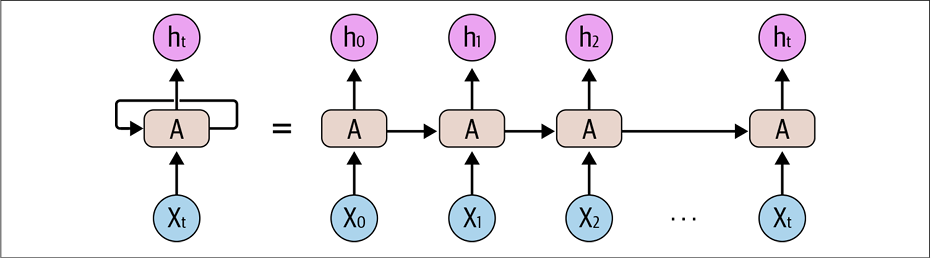
\includegraphics[width=\textwidth]{imagenes/Cap 2/rnn.png}
	\caption{RNN}
	\label{fig:RNN}
	\cite{sowmya_practical_npl}
\end{figure}

Las RNNs son poderosas y funcionan muy bien para resolver muchas tareas de NLP, como clasificación
de texto, reconocimiento
de entidad, traducción automática, etc. También se pueden utilizar para generar texto, por ejemplo
para predecir la
siguiente palabra de se va a escribir de acuerdo al contexto de lo que ya se escribió.

A pesar de su versatilidad y capacidad, las RNNs sufren de ciertas limitaciones por contar con
memoria temporal, por lo
tanto no se desempeñan óptimamente para textos con largos contextos. Pero para estos existen
variaciones optimizadas para
memoria de largo plazo(LSTMs).

\subsection{Redes Neuronales Convencionales(CNN)}
Las CNNs por sus siglas en Inglés o Redes Neuronales Convolucionales son muy populares y muy
frecuentemente usadas para
para aplicaciones como clasificación de imágenes, reconocimiento de vídeo, etc. Las CNNs también
vieron éxito en NLP,
específicamente en clasificación de texto. Se puede reemplazar una palabra de una oración de un
texto por un vector
palabra, y estos a su vez ser colocados en una matriz para poder ser tratados de manera similar a
una imagen.

\begin{figure}[H]
	\centering
	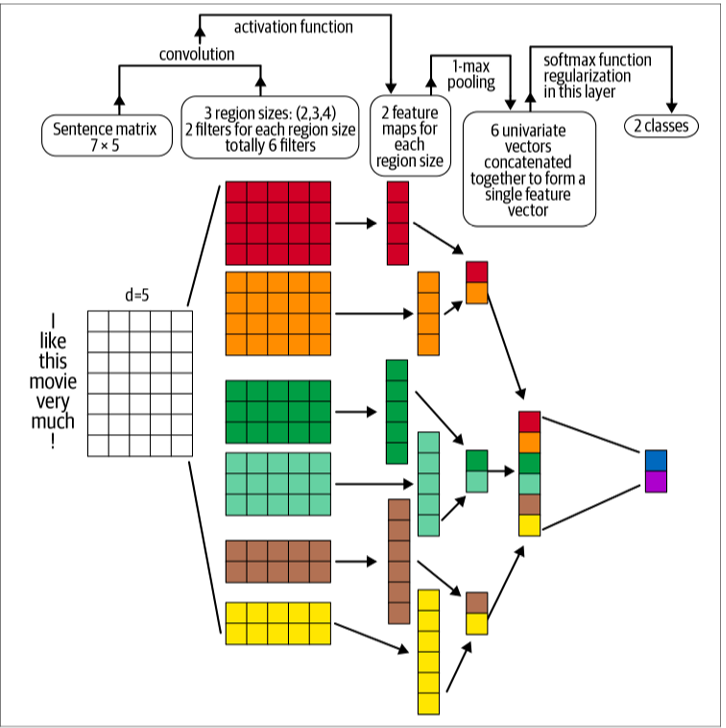
\includegraphics[width=0.8\textwidth]{imagenes/Cap 2/cnn.png}
	\caption{Diagrama de CNN}
	\label{fig:CNN}
	\cite{sowmya_practical_npl}
\end{figure}

\subsection{Tranformadores}

Los trasformadores son la última innovación en lo que respecta a modelos basados en DL para NLP.
Los
modelos de transformadores obtuvieron avances en la mayoría de las tareas de NLP en los últimos
años. \\
Estos modelan el contexto textual pero no de manera secuencial. Dada una palabra en una entrada de
texto, se
prefiere mirar las demás palabras vecinas en el texto y representar cada palabra de acuerdo a el
contexto
de las demás. Por ejemplo si el contexto habla de finanzas, entonces "banco" probablemente
representaría una
institución financiera. Por otro lado en el contexto de un río, estaría relacionado con un
montículo de tierra.
Recientemente, los transformadores han sido utilizados para transferir aprendizaje con flujos de
pequeñas tareas,
La transferencia de aprendizaje es una técnica en IA en la cual lo que se aprendió en resolver un
problema es
aplicado para resolver problemas similares.

\begin{figure}[H]
	\centering
	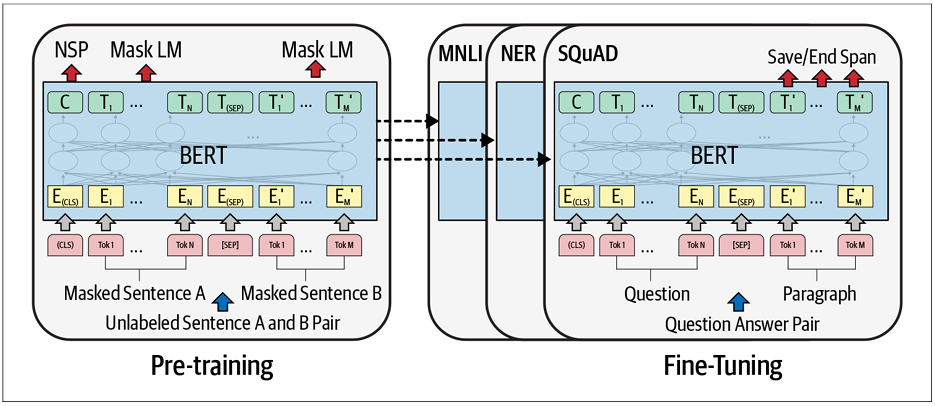
\includegraphics[width=0.8\textwidth]{imagenes/Cap 2/tranformers.png}
	\caption{Diagrama de un Transformador}
	\label{fig:Transformadores}
	\cite{sowmya_practical_npl}
\end{figure}

\subsection{Autoencoders}
Los autoencoders son otro tipo de red neuronal utilizadas principalmente para aprender a
representar la
entrada de forma comprimida en un vector. Por ejemplo, si queremos representar unas palabras en un
vector,
podemos aprender a mapear el texto en vectores y luego remapear para reconstruir la entrada
original.
Esto es una forma de aprendizaje no supervisado ya que no se necesitan datos anotados para el
entrenamiento.\\

\begin{figure}[H]
	\centering
	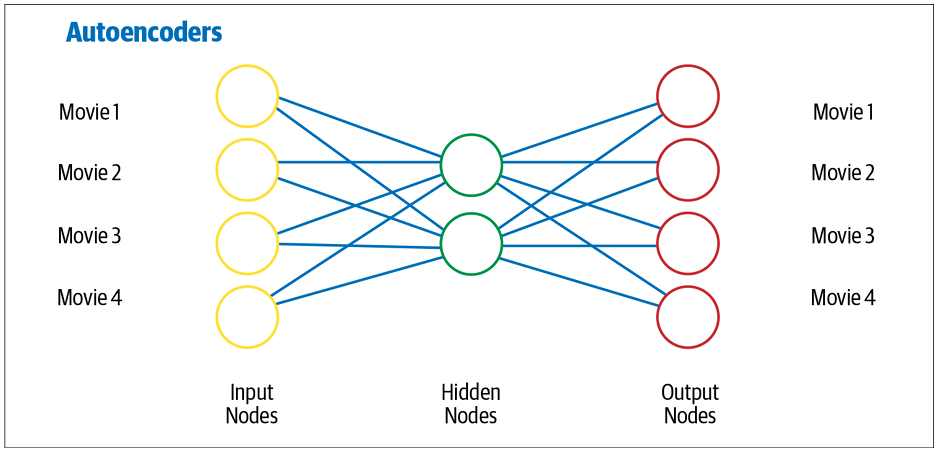
\includegraphics[width=0.8\textwidth]{imagenes/Cap 2/autoencoder.png}
	\caption{Representacion de un autoencoder}
	\label{fig:autoencoder}
	\cite{sowmya_practical_npl}
\end{figure}

%comparacion de metodos 

% TODO agregar aplicaciones 

\section{Chatbots}
% conceptos mas específicos
%---data adquisitcition

%----extraccion de texto

%----preprosesado

%----feature engineeniring 

%----modeling 

%---evaluation

%----post modelign 

\subsection{Concepto}
Los chatbots son programas que imitan la conversación humana utilizando la Inteligencia
Artificial.\cite{UniversityRelatedFAQS}
\subsection{Características}
Existen diferentes tipos de chatbots, clasificados según su complejidad, objetivos o funciones,
pero todos ellos cuentan con las siguientes cualidades según Nicol Radziwill y Morgan Benton
\cite{evaluating_quality}
\begin{itemize}
	\item Rendimiento: se refiere a la eficiencia en la asignación de funciones y a la robustez que
	      tienen en cuanto a la manipulación y a las entradas inesperadas.
	\item Funcionalidad: es capaz de interpretar, responder y ejecutar	correctamente las tareas
	      demandadas.
	\item Humanidad: la conversación con el chatbot debe ser natural, lo mas parecida a la humana.
	\item Ética: genera confianza, respeta y protege la dignidad, y la privacidad de los usuarios.
	\item Accesibilidad: se encuentra disponible cuando el usuario quiera usarlo, además se refiere
	      a que es capaz de detectar intenciones y significados
\end{itemize}
% documentación de rasa como referencia

\subsection{Aplicaciones}
Se pueden mencionar dos tipos de aplicaciones:
\begin{itemize}
	\item Asistentes Personales Virtuales: ofrecen servicios a los usuarios a través de texto o
	      voz. Ejemplos: Siri(Apple), Google Assistant, Alexa (Amazon) y Cortana (Microsoft)
	\item Bots para el consumo específico: sus aplicaciones son muy variadas, puede utilizarse en
	      el transporte, la salud, el clima, entretenimiento o incluso en la educación.
\end{itemize}
\subsection{Arquitectura}
Para el diseño adecuado de cualquier sistema la mejor solución es dividirla en varias partes o
subsistemas de acuerdo a un estándar.
En la figura \ref{fig:Arquitectura} se puede ver que existen dos bloques bien definidos, al primero
se lo llama 'lado del cliente' que es la parte que interactúa con los usuarios; y el segundo bloque
es el 'lado del servidor' encargado de procesar las peticiones del cliente.\\
\begin{figure}[h]
	\centering
	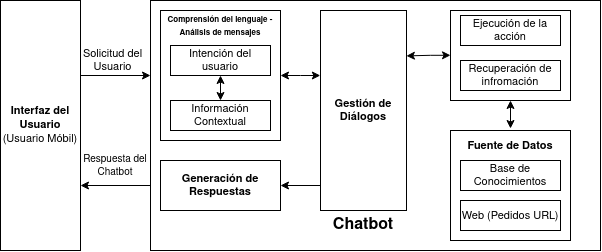
\includegraphics[width=\textwidth]{imagenes/Cap 2/Arquitectura.png}
	\caption{Arquitectura de los Chatbots}
	\label{fig:Arquitectura}
\end{figure}
\indent El  proceso inicia en la interfaz de usuario cuando el cliente realiza una solicitud, ésta
es analizada en el bloque componente de comprensión de lenguaje, aquí se extrae toda la información
necesaria y se deduce las intenciones del usuario.\\
\indent Una vez que el chatbot llegue a la mejor interpretación que puede, ejecuta las acciones
solicitadas o recupera la información de su fuente de datos, que puede ser una base de datos propia
o datos externos accedidos a través de APIs.\\
\indent Posteriormente se generan las respuestas lo más parecidas a las que daría una persona
humana, para ello utiliza la información de intención y contexto proveída por el componente de
análisis de mensajes del usuario.\\
\indent El componente de gestión de diálogo se encarga de solicitar información faltante,
aclaraciones y hacer preguntas de seguimiento.\cite{Overview_of_chatbots}

\subsection{Plataformas de desarrollo}
\begin{itemize}
	\item DialogFlow:
	      Es la plataforma de desarrollo de chatbots de Google, permite una fácil integración a
	      aplicaciones móviles y web, también facilita bastante el diseño de la interfaz de usuario.\\
	      Admite como entrada texto y voz, es capaz de responder a los clientes con texto o voz
	      sintética.\\
	      Existen dos versiones, Dialogflw CX utilizado para agentes grandes o muy avanzados y
	      Dialogflow ES que es la versión estándar, ésta cuenta con una versión gratuita.\\
	      El precio varia según la versión elegida y el tipo de entrada, Dialogflow ES cobra 0.002
	      USD por cada solicitud realizada por texto y 0.0065 USD si la entrada es un audio de hasta 15
	      segundos.\cite{Dialogflow}
	\item IBM Watson:
	      IBM Watson  permite a los usuarios integrar sus chatbots en cualquier canal, sea web,
	      aplicaciones o incluso una llamada.\\
	      Es capaz de aprender los vocabularios de la industria,	términos coloquiales o dialectos
	      regionales, admite entradas de voz y también de texto. \\
	      Está diseñada para aprender sobre el camino, proporciona herramientas para detectar las
	      tendencias y estas ayudan a asignar recursos de forma mas eficiente y eficaz.\\
	      No es necesario escribir ni una sola linea de código ya que utiliza un entorno de 'arrastre
	      y suelte' para construir los diálogos y una vez que lo adaptemos a nuestras necesidades, fácilmente
	      lo incorporamos a la app con 'copiar y pegar'.\cite{IBMCloud2020}\\
	      Cuenta con tres versiones: la versión mas básica, Lite, es gratuita pero muy limitada en
	      sus funcionalidades.
	      Luego vienen las versiones de paga, Plus y Enterprise con precios que van desde los 140 USD
	      por mes.\cite{IBM_Price}
	\item Amazon Lex:
	      Amazon Lex es la propuesta del gigante tecnológico Amazon, sirve para diseñar, crear,
	      probar e implementar interfaces de conversación en las aplicaciones.\\
	      Reconoce tanto entradas de texto como de voz, gestiona el contexto de las conversaciones de
	      forma nativa y también permite una gran fidelidad en las interacciones de habla telefónica.\\
	      La integración con plataformas se realiza de forma muy sencilla desde la consola de Amazon
	      Lex , permite aplicaciones web, móviles y los servicios propios de Amazon como Amazon Kendra,
	      Amazon Polly o AWS Lambda.\\
	      Los precios varían según el tipo de servicio solicitado, El mas básico 'Interacción de
	      respuesta y solicitud' cobra 0,004 USD por solicitud de voz y 0,00075 USD por solicitud de
	      texto.\cite{Amazon_Lex}
	\item RASA Open Source:
	      Es una plataforma de código abierto que proporciona procesamiento de lenguaje natural para
	      convertir los mensajes de los usuarios en intenciones y entidades que los chatbots entienden,
	      permite la gestión de los diálogos basándose en los mensajes de los usuarios y el contexto de la
	      conversación.\\
	      La integración a las aplicaciones mas comunes de mensajes y a los canales de voz se puede hacer
	      de forma muy sencilla con los conectores ya incorporados, para conectar a las demás aplicaciones
	      móviles o web se deben personalizar los conectores.\\
	      RASA también tiene una versión de paga denominada RASA Enterprise, utilizada para el despliegue
	      a escala, su precio varía de acuerdo a las necesidades de la organización y del
	      proyecto.\cite{Rasa}
	\item Chatterbot:
	      Chatterbot es una librería de Python que facilita la automatización de respuestas mediante
	      distintos algoritmos de aprendizaje automático, esto permite que una instancia de agente mejore su
	      propio conocimiento de las posibles respuestas a medida que interactúa con humanos y otras fuentes
	      de datos informativos\\
	      Cada vez que un usuario introduce una frase, la librería guarda el texto que ha introducido y
	      el texto al que responde la frase. A medida que ChatterBot recibe más entradas, aumenta el número
	      de respuestas que puede dar y la precisión de cada respuesta en relación con la declaración
	      introducida.\\
	      Se puede integrar a las aplicaciones mediante APIs, además ChatterBot tiene soporte directo
	      para la integración con el ORM de Django, esto facilita bastante para crear las páginas
	      conversacionales.\cite{Chatterbot}\\
\end{itemize}

\indent Haciendo una comparación entre todas las herramientas analizadas, vemos que la creación de
los chatbots con Dialogflow, IBM Watson y Amazon Lex es mucho mas sencilla, ya que tienen una
madurez tecnológica muy alta, gran soporte y las interfaces son muy intuitivas, además no requieren
de mucha programación. La mayor desventaja es que las versiones que cuentan con todas las
funcionalidades son de paga, y las versiones gratuitas son muy limitadas y básicas, por lo que
descartamos estas tres opciones.\\
\indent En cuanto a Chatterbot y RASA, la curva de aprendizaje puede ser un poco mayor porque no
utilizan interfaces gráficas, todo es programado con Python, un lenguaje muy versátil que cuenta
con numerosas librerias, esto permite tener mayor control sobre los chatbots porque se pueden
manipular todos los ficheros y modificar las configuraciones, Si bien ambos están muy bien
documentados, RASA destaca de Chatterbot por su comunidad, cuenta incluso con un foro donde
participan los desarrolladores y usuarios dispuestos a brindar ayuda a todo aquel que las
necesite.\\
\indent Teniendo en cuenta que no contamos con experiencia en el desarrollo de chatbots, se valora
de sobremanera la comunidad, documentación y tutoriales con los que cuenta RASA, además que permite
la integración con distintas plataformas y el lenguaje de programación que utiliza (Python) es de
nuestro conocimiento, es por eso que concluimos con que RASA es una buena elección para llevar a
cabo este proyecto.
